% Ensure included PDFs (banners) with newer versions embed without warnings
\pdfminorversion=7
\documentclass[aspectratio=169]{beamer}

\makeatletter
% Make LaTeX find theme .sty files in Template
\def\input@path{{../Template/}}
\makeatother
\usepackage{graphicx}
% Make graphics (including banner PDFs) resolvable without TEXINPUTS
\graphicspath{{../Template/}{../Template/banners/}{../../Common_Images/}}

%================================================================%
% Theme and Package Setup
%================================================================%
\usetheme{ucl}
\setbeamercolor{banner}{bg=darkpurple}

% Navigation and Footer
\setbeamertemplate{navigation symbols}{\vspace{-2ex}}
\setbeamertemplate{footline}[author title date]
\setbeamertemplate{slide counter}[framenumber/totalframenumber]

\usepackage[utf8]{inputenc}
\usepackage[british]{babel} % British spelling
\usepackage{amsmath, amssymb, amsthm}
\usepackage{graphicx}
\usepackage{tikz}
\usetikzlibrary{calc, positioning, arrows.meta, shapes.geometric, trees, backgrounds, shapes.misc, graphs, quotes, shadows, fit, patterns} 
\usepackage{pgfplots}
\pgfplotsset{compat=1.17}
\usefonttheme{professionalfonts}
\usepackage{eulervm}
\usepackage{listings}
\usepackage{algorithm}
\usepackage{algpseudocode}
\usepackage{xcolor}
\usepackage{subcaption}

% Define custom colours
\makeatletter
\@ifundefined{color@stone}{%
    \definecolor{stone}{gray}{0.95}%
}{}
\makeatother
\definecolor{darkgreen}{rgb}{0.0, 0.5, 0.0}
\definecolor{uclblue}{cmyk}{1,0.24,0,0.64}
\definecolor{uclred}{cmyk}{0,1,0.62,0}

\setbeamercovered{transparent}

% Define theoremblock
\makeatletter
\newenvironment<>{theoremblock}[1]{%
    \begin{block}#2{#1}%
}{\end{block}}
\makeatother

% Section divider slides
\AtBeginSection[]{
  \begin{frame}
    \frametitle{\textbf{\Large\insertsectionhead}}
    \begin{center}
        \huge\textbf{\insertsectionhead}
    \end{center}
  \end{frame}
}

% Maths Macros
\newcommand{\U}{\mathcal{U}}
\newcommand{\V}{\mathcal{V}}
\newcommand{\Z}{\mathcal{Z}}
\newcommand{\R}{\mathbb{R}}
\newcommand{\E}{\mathbb{E}}
\newcommand{\ip}[2]{\langle #1, #2 \rangle}
\newcommand{\norm}[1]{\| #1 \|}
\DeclareMathOperator*{\argmin}{argmin}
\DeclareMathOperator{\prox}{prox}
\DeclareMathOperator{\dom}{dom}
\DeclareMathOperator{\supremum}{sup}
\DeclareMathOperator{\sign}{sign}

\title{Continuous Dynamics and Variational Networks}
\subtitle{Lecture 1: Deep Learning as Continuous Dynamical Systems \& Optimal Control}
\author[Martin Benning (University College London)]{Martin Benning}
\date[COMP0263]{COMP0263 -- Solving Inverse Problems with Data-Driven Models \\[1cm] 3rd March 2026}
\institute[]{University College London}

\begin{document}

% --- Title Frame ---
\begin{frame}
  \titlepage
\end{frame}

% --- Outline ---
\begin{frame}{Lecture Overview}
    \tableofcontents
\end{frame}

\section{Introduction \& The Memory Bottleneck}

\begin{frame}{Recap: Algorithm Unrolling}
    In Week 5, we explored the paradigm of \textbf{algorithm unrolling}:
    
    \begin{itemize}
        \item We bridged classical iterative optimisation with deep learning.
        \item By unrolling a finite number of iterations (e.g., proximal gradient descent), we replaced hand-crafted parameters with \emph{learnable components}.
        \item This created architectures connected to the physics of inverse problems while leveraging data-driven expressivity.
    \end{itemize}
\end{frame}

\begin{frame}{The Computational Wall}
    However, unrolling generic optimisation algorithms leaves several practical questions unanswered.\vspace{1em}
    
    As we increase the number of unrolled iterations (layers) to improve accuracy, we hit a severe computational bottleneck: \textbf{Backpropagation Through Time (BPTT)}.
\end{frame}

\begin{frame}{Memory Scaling in 3D Inverse Problems}
    \begin{theoremblock}{The BPTT Limitation}
        Evaluating gradients via BPTT requires storing the intermediate activations of \emph{every single layer} in memory during the forward pass.
    \end{theoremblock}
    \vspace{1em}
    
    \begin{itemize}
        \item Memory requirements scale \textbf{linearly} with network depth.
        \item For large-scale 3D inverse problems (e.g., MRI, CT), this quickly exceeds the memory capacity of modern hardware (GPUs/TPUs).
    \end{itemize}
\end{frame}

\begin{frame}{The Perspective Shift}
    Furthermore, relying on discrete iterative steps obscures the underlying continuous physics of the learning process.\vspace{1em}
    
    \textbf{The Solution:} We initiate a profound shift in perspective \cite{e2017proposal, haber2017stable}.
    \begin{itemize}
        \item We will reframe deep learning not as a sequence of discrete algebraic layers, but as a problem of \textbf{continuous dynamical systems}.
        \item By taking the infinitesimal limit of deep residual networks, we arrive at continuous-time Ordinary Differential Equations (ODEs).
    \end{itemize}
\end{frame}

\section{The Continuous Limit}

\begin{frame}{Generic Layer Transitions}
    To understand this continuous limit, let us examine the mathematical structure of a single discrete neural network layer.\vspace{1em}
    
    A generic layer transition is typically modelled as
    $$u^{l+1}=G\left(h(u^l)+\mathcal{F}(u^l,\Theta_l)\right)$$
    
    \begin{itemize}
        \item $u^l \in \mathbb{R}^d$: Input state vector at layer $l$.
        \item $\Theta_l$: Learnable parameters (weights, biases).
        \item $\mathcal{F}$: Parameterised mapping (e.g., convolution or affine operations followed by nonlinear activation functions) representing the core transformation block.
        \item $G, h$: Mapping functions (e.g., non-linear activations, normalisation).
    \end{itemize}
\end{frame}

\begin{frame}{The Exploding/Vanishing Gradient Problem}
    When stacking generic layers to create exceptionally deep networks, a critical numerical pathology emerges.
    
    For a deep network to remain trainable via gradient descent, the mapping from layer $l$ to $l+1$ must remain stable. 
    
    Mathematically, the gradient of the transition must be close to the identity matrix, i.e.,
    $$\nabla G\nabla h\sim I$$
    
    If eigenvalues deviate significantly from one, perturbations will either decay to zero (\textbf{vanishing}) or grow exponentially (\textbf{exploding}).
\end{frame}

\begin{frame}{ResNets as Stable Additive Perturbations}
    \textbf{Residual Networks (ResNets)} better fulfil this stability condition.\vspace{1em}
    
    By setting $G(x) = x$ and $h(x) = x$, the update rule becomes a simple additive perturbation to the identity map
    $$u^{l+1}=u^l+\mathcal{F}(u^l,\Theta_l) \, . $$
    
    This ensures that $\nabla_{u^l}u^{l+1}=I+\nabla_{u^l}\mathcal{F}(u^l,\Theta_l)$, regularising the flow of gradients and allowing for the training of networks with hundreds of layers.
\end{frame}

\begin{frame}{Deriving the Continuous ODE (1/2)}
    The discrete ResNet transition reveals a deep connection to numerical analysis. Let us rewrite the update rule by introducing an artificial step size $\Delta t = 1$:
    
    $$\frac{u^{l+1}-u^l}{\Delta t}=\mathcal{F}(u^l,\Theta_l)$$
    
    \begin{theoremblock}{Forward Euler Discretisation}
        This algebraic manipulation shows that the ResNet layer is exactly the \emph{forward Euler discretisation} of a continuous ordinary differential equation.
    \end{theoremblock}
\end{frame}

\begin{frame}{Deriving the Continuous ODE (2/2)}
    We imagine the discrete layer index $l$ mapping to a continuous time equivalent $t_l = l \Delta t$.\vspace{1em}
    
    If we allow the step size $\Delta t \to 0$ and the number of layers to approach infinity (keeping the total "network time" horizon $T$ fixed):
    \begin{itemize}
        \item The hidden states $u^l$ transition into a \textbf{continuous trajectory} $u(t)$.
        \item The discrete parameters $\Theta_l$ become a \textbf{continuous control variable} $\Theta(t)$.
    \end{itemize}
    \vspace{1em}
    \small{Note: See earlier works unifying ODEs and deep learning, e.g., \cite{e2017proposal, haber2017stable, benning2019deep}.}
\end{frame}

\begin{frame}{Initial Value Problem Formulation}
    By taking the infinitesimal limit, the difference quotient becomes a time derivative, governed by the initial value problem
    
    $$\frac{d}{dt}u(t)=\mathcal{F}\left(u(t),\Theta(t)\right)\quad\text{for }t\in[0,T] \, .$$
    
    \textbf{Initial Condition:} $u(0) = u_0$ (where $u_0$ is the input data).\vspace{1em}
    
    Here, $\Theta(t)$ represents the time-dependent network weights and biases acting over a fixed network time horizon $T$.
\end{frame}

\begin{frame}{Overcoming Numerical Instability}
    Framing network architectures as discretised ODEs provides a rigorous mathematical framework for designing stable architectures.\vspace{1em}
    
    By interpreting the forward pass as the integration of an ODE:
    \begin{itemize}
        \item We ensure the learning problem remains well-posed.
        \item If the vector field $\mathcal{F}(u, \Theta(t))$ is appropriately constrained, the flow remains bounded and stable from $u(0)$ to $u(T)$.
        \item This continuous perspective can overcome the numerical instabilities inherent in standard learning algorithms.
    \end{itemize}
\end{frame}

\section{Deep Learning as Continuous Optimal Control}

\begin{frame}{Transforming Supervised Learning}
    By formally interpreting the neural network as a continuous dynamical system, the supervised training process is mathematically transformed into an \textbf{optimal control problem} \cite{benning2019deep, e2017proposal}.
    
    \vspace{1em}
    Instead of finding a discrete set of parameters, our objective is to find an \emph{optimal continuous control trajectory} $\Theta(t)$ that steers the dynamical system to a desired terminal state $u(T)$ at time $t=T$.
\end{frame}

\begin{frame}{Advantages of the Continuous Perspective}
    This continuous perspective offers several profound advantages over the discrete layer-by-layer view:
    
    \begin{enumerate}
        \item \textbf{Decoupling:} It allows us to decouple the learning problem (finding the optimal continuous trajectory) from the discretisation (how we numerically compute the forward pass).
        \item \textbf{Mathematical Rigour:} It connects deep learning to established optimal control theory, granting access to powerful analytical tools like the Pontryagin Maximum Principle.
    \end{enumerate}
\end{frame}

\begin{frame}{Defining the Cost Functional}
    In classical deep learning, we minimise an empirical risk function over learnable parameters. In our continuous framework, this is generalised via a cost functional over the entire time horizon $[0, T]$.
    
    \begin{theoremblock}{The Generic Cost Functional}
    $$\min_{\Theta,u}\left\{\mathcal{J}(u(T),\Theta):=\mathcal{M}(u(T))+\int_0^T\mathcal{R}(u(t),\Theta(t))\,dt\right\}$$
    \end{theoremblock}
    
    \begin{itemize}
        \item $\mathcal{M}(u(T))$: \textbf{Terminal Cost} (how well the final state performs the task).
        \item $\mathcal{R}(u(t), \Theta(t))$: \textbf{Running Cost} (regularising the control parameters over time).
    \end{itemize}
\end{frame}

\begin{frame}{The Continuous State Evolution Constraint}
    This minimisation is subject to the fundamental ODE constraint governing the continuous state evolution
    
    $$\frac{d}{dt}u(t)=\mathcal{F}\left(u(t),\Theta(t)\right)\quad\text{for }t\in(0,T] \, , $$
    
    with initial condition $u(0) = u_0$.
    \vspace{1em}
    
    Here, $u(t) \in \mathcal{U}$ belongs to the state space, and the control sequence $\Theta(t) \in \mathcal{P}$ belongs to an admissible parameter class.
\end{frame}

\begin{frame}{Example: Training a Classifier on Data}
    Suppose we have a dataset of $m$ input-output pairs $(x_i, y_i) \in \mathbb{R}^d \times \{0,1\}$. We construct the terminal cost function $\mathcal{M}$ (empirical risk) and a running cost $\mathcal{R}$ (Tikhonov regularisation) via
    \begin{align*}
        \mathcal{M}(u(T))&:=\frac{1}{m}\sum_{i=1}^m\left|\mathcal{C}\left(Wu_i(T)+\mu\right)-y_i\right|^2\\
        \mathcal{R}(u(t),\Theta(t))&:=\frac{\lambda}{2}\|\Theta(t)\|_2^2
    \end{align*}
    
    where $\mathcal{C}(z) = 1/(1 + \exp(-z))$ is the standard logistic sigmoid function. This yields the \textbf{Optimal Control Problem}
    $$\min_{\Theta,u,W,\mu}\left\{\frac{1}{m}\sum_{i=1}^m\left|\mathcal{C}\left(Wu_i(T)+\mu\right)-y_i\right|^2+\frac{\lambda}{2}\int_0^T\|\Theta(t)\|_2^2\,dt\right\} \, , $$
    subject to $\frac{d}{dt}u_i(t) = \mathcal{F}(u_i(t), \Theta(t))$ and $u_i(0) = x_i$.
\end{frame}

\begin{frame}{Visualising the Continuous Transformation}
    To visualise this continuous transformation, we can apply this optimal control framework to standard 2D binary classification tasks, such as separating interleaved spirals.
    
    \begin{figure}[htpb]
        \centering
        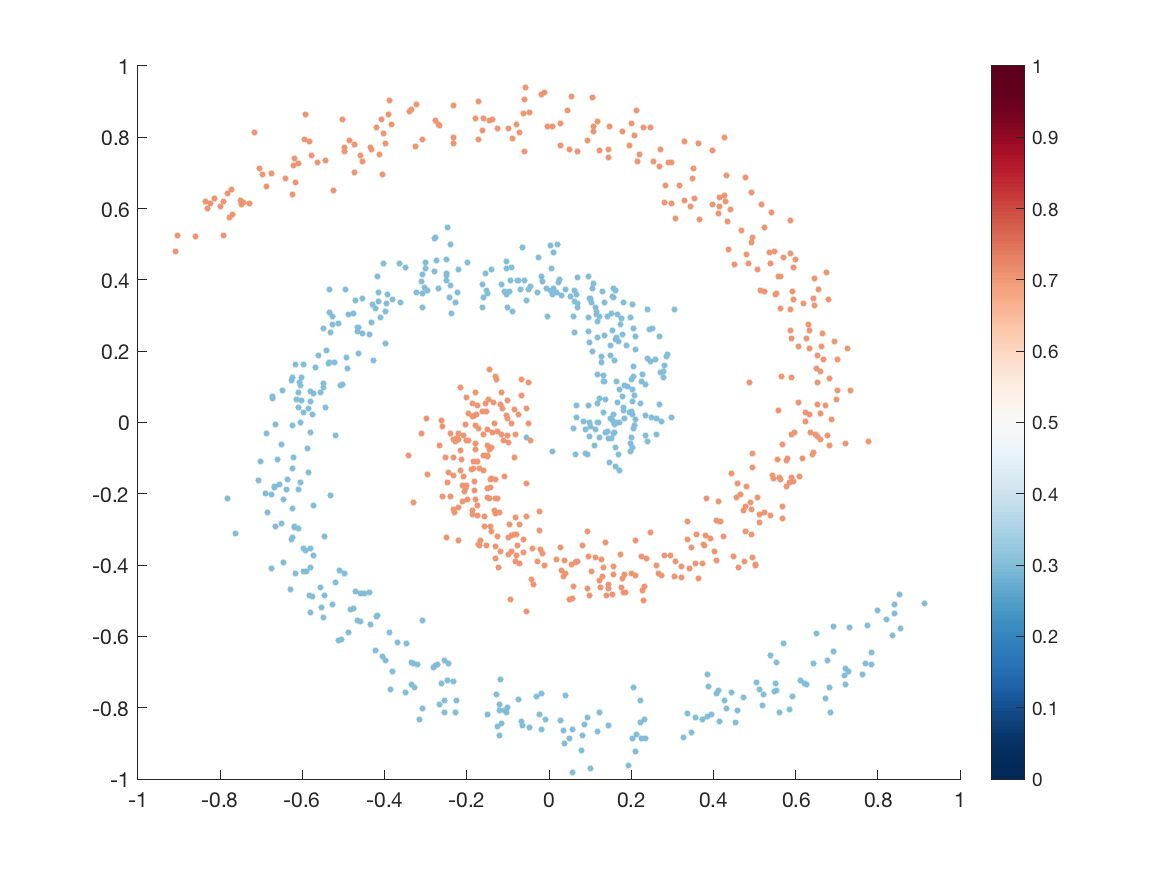
\includegraphics[width=0.38\textwidth]{../Common_Images/optimalcontrol/example_spiral2d} 
        \caption{A 2D binary classification toy dataset (spirals). The network learns a flow that disentangles the two classes over the time horizon $T$.}
    \end{figure}
\end{frame}

\begin{frame}{Visualising the Flow}
    As the continuous network time $t$ progresses to $T$, the learned optimal control trajectory $\Theta(t)$ dynamically transforms the state space, warping the geometry of the data points until they are linearly separable.
    
    \begin{figure}[htpb]
        \centering
        \begin{subfigure}[b]{0.24\textwidth}
            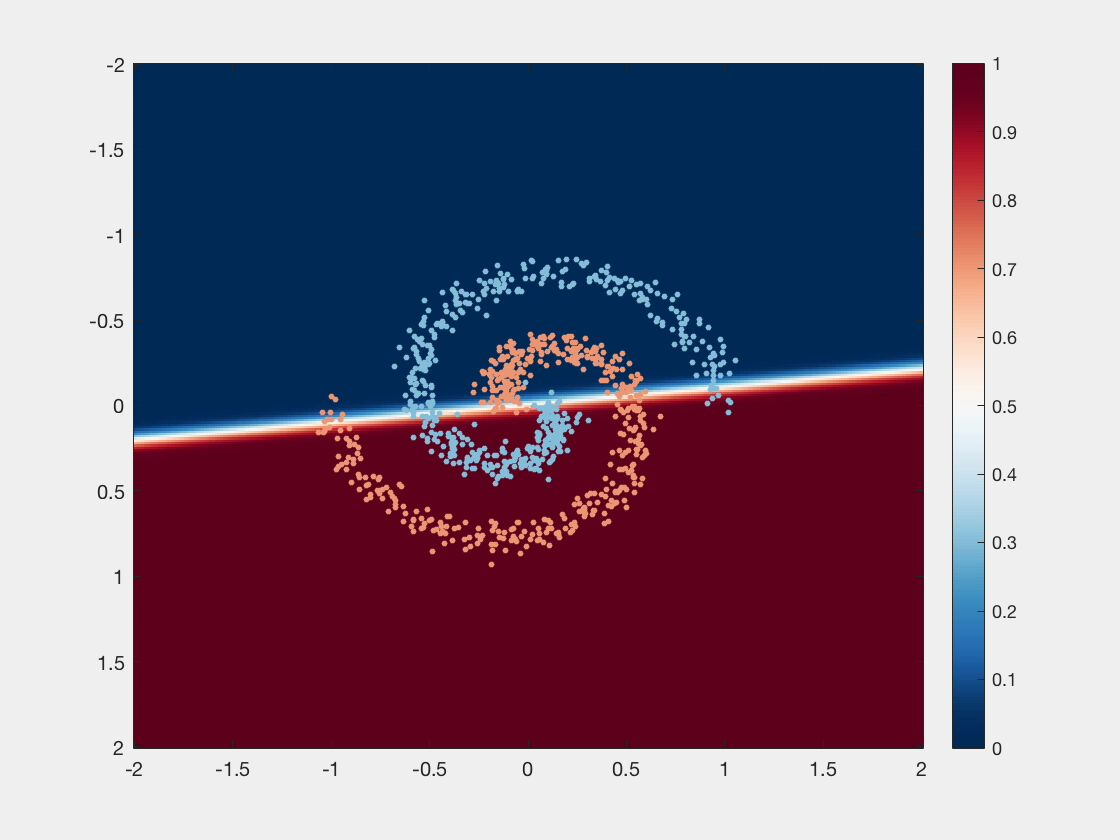
\includegraphics[width=\textwidth]{../Common_Images/optimalcontrol/ResNet_squared_seed1_video_01}
            \caption{$t=0$}
        \end{subfigure}
        \hfill
        \begin{subfigure}[b]{0.24\textwidth}
            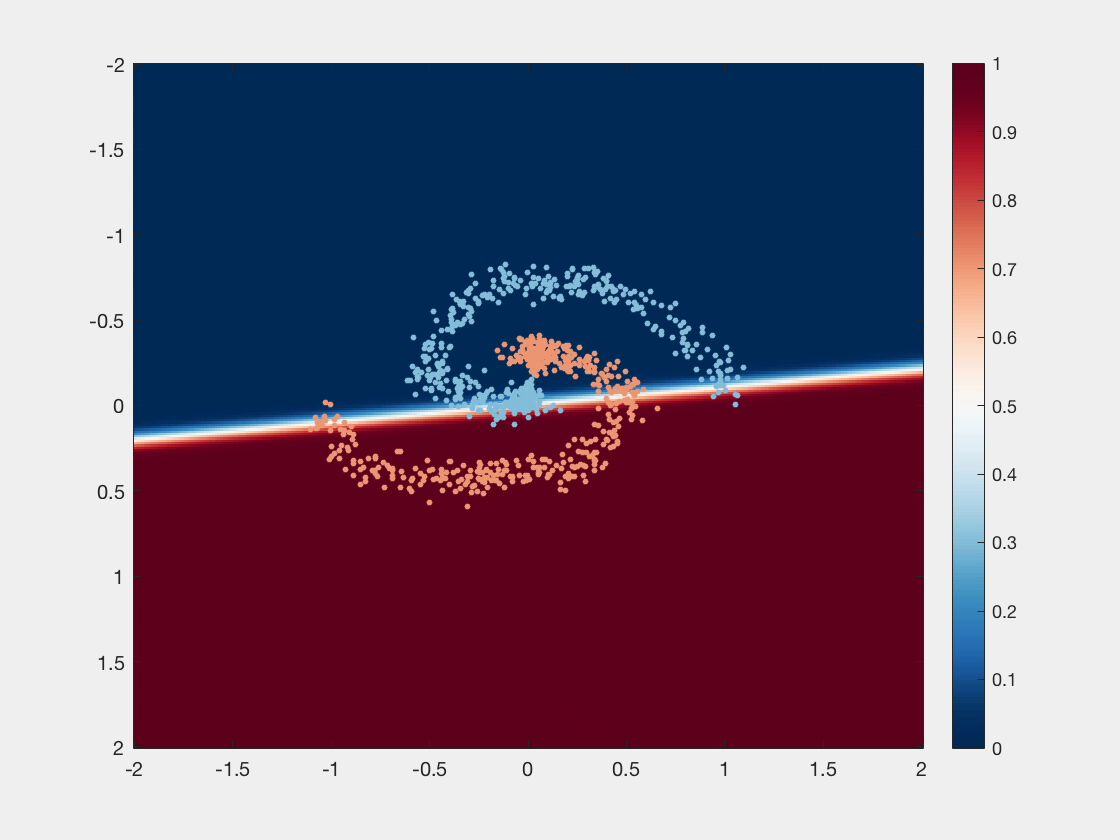
\includegraphics[width=\textwidth]{../Common_Images/optimalcontrol/ResNet_squared_seed1_video_08}
            \caption{$t \approx T/3$}
        \end{subfigure}
        \hfill
        \begin{subfigure}[b]{0.24\textwidth}
            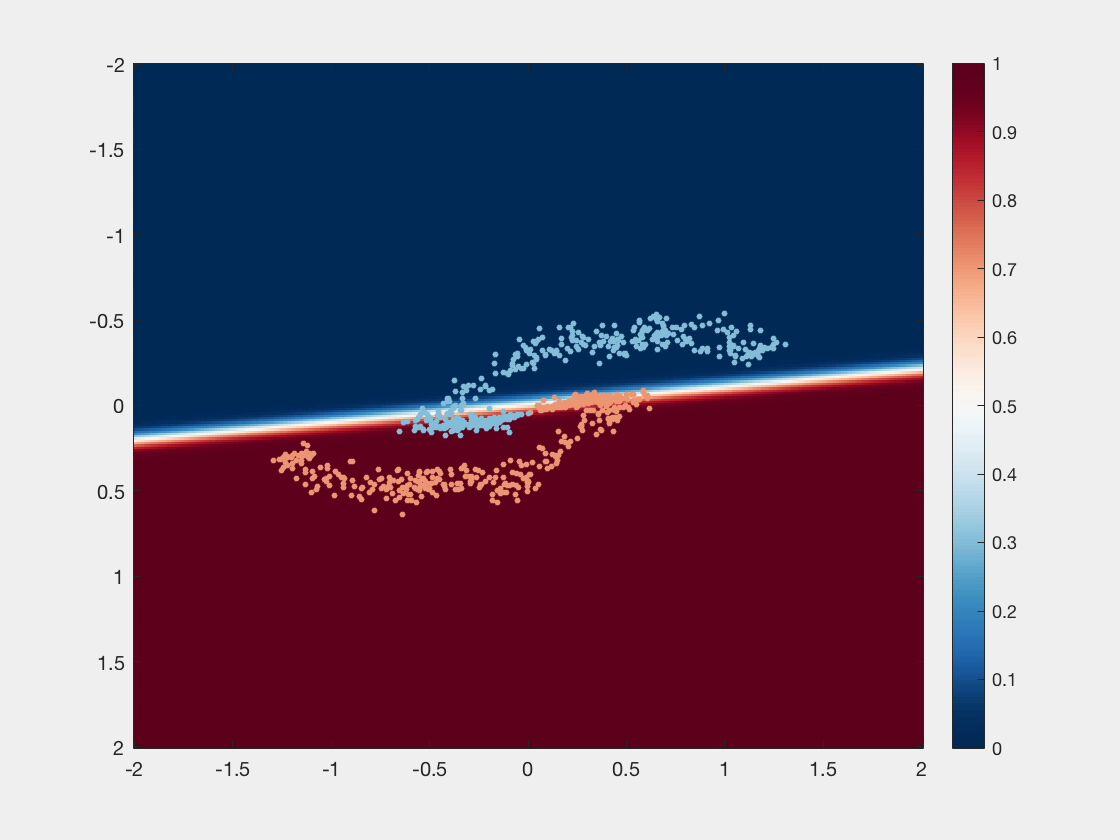
\includegraphics[width=\textwidth]{../Common_Images/optimalcontrol/ResNet_squared_seed1_video_15}
            \caption{$t \approx 2T/3$}
        \end{subfigure}
        \hfill
        \begin{subfigure}[b]{0.24\textwidth}
            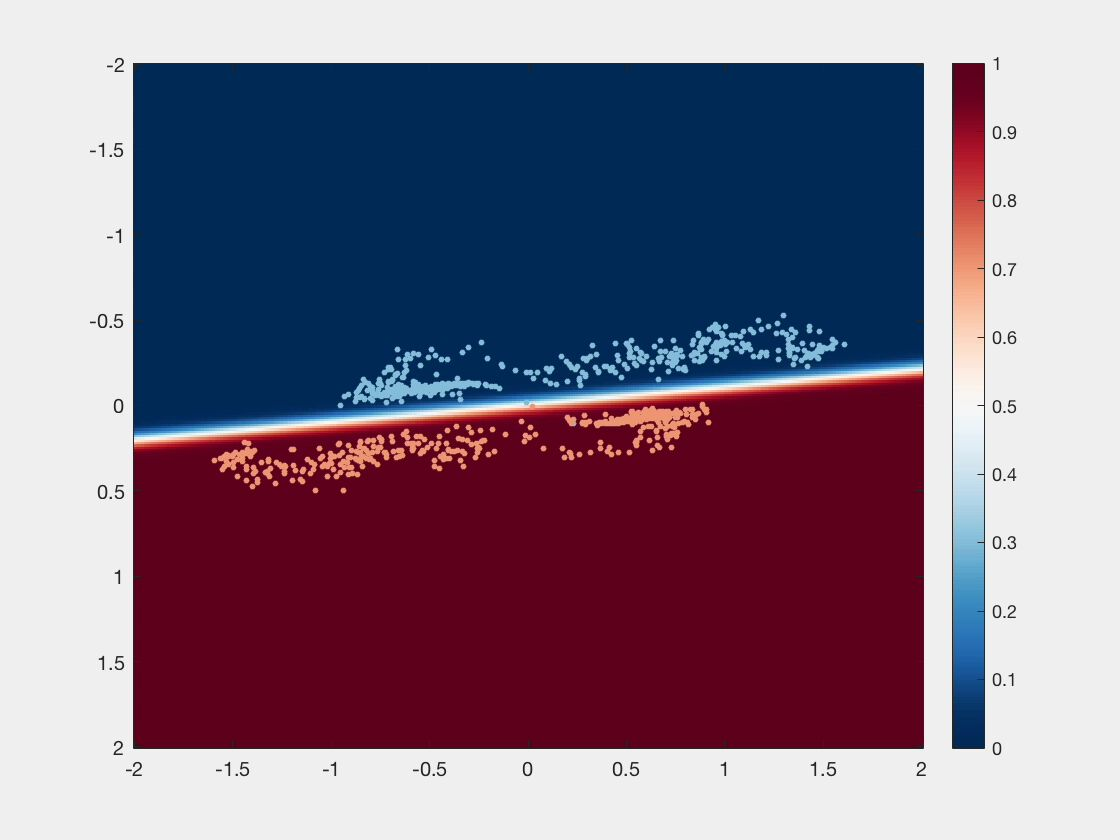
\includegraphics[width=\textwidth]{../Common_Images/optimalcontrol/ResNet_squared_seed1_video_21}
            \caption{$t=T$}
        \end{subfigure}
        \caption{Progression of state space transformation across the continuous horizon using a ResNet flow.}
    \end{figure}
\end{frame}

\section{The Lagrangian \& First-Order Optimality}

\begin{frame}{Gradient-Based Optimisation}
    To perform gradient-based numerical optimisation, we need to know how the final cost $\mathcal{J}$ reacts to continuous changes in the control signal $\Theta(t)$.\vspace{1em}
    
    Similar to previous weeks, we employ \textbf{Lagrange multipliers}. 
    \vspace{1em}
    
    This elegantly reformulates the constrained optimal control problem into an \emph{unconstrained saddle-point problem}.
\end{frame}

\begin{frame}{The Adjoint State $p(t)$}
    We introduce a continuous-time Lagrange multiplier $p(t) \in \mathcal{U}^\ast$, referred to in optimal control terminology as the \textbf{adjoint state} (or co-state). \vspace{1em}
    
    The Lagrangian functional $\mathcal{L}(u, \Theta, p)$ is defined by appending the ODE constraint to the generic cost functional via an $L^2$-inner product integrated over the entire time horizon.
\end{frame}

\begin{frame}{Formulating the Unconstrained Lagrangian}
    Writing this in mathematical terms, we define
    \begin{align*}
        \mathcal{L}(u,\Theta,p)&:=\mathcal{M}\left(u(T)\right)+\int_0^T\mathcal{R}\left(u(t),\Theta(t)\right)\,dt\\
        &\quad-\int_0^T\left\langle p(t),\frac{d}{dt}u(t)-\mathcal{F}\left(u(t),\Theta(t)\right)\right\rangle_{\mathcal{U}}\,dt \, .
    \end{align*}
    
    To make it easier to take derivatives with respect to $u(t)$, we must isolate $u(t)$ from its time derivative.
\end{frame}

\begin{frame}{Integration by Parts}
    We isolate $u(t)$ by applying integration by parts to the first half of the constraint integral to obtain
    
    \begin{theoremblock}{Integration by Parts}
    $$\int_0^T\left\langle p(t),\frac{d}{dt}u(t)\right\rangle_{\mathcal{U}}\,dt=\langle p(T),u(T)\rangle_{\mathcal{U}}-\langle p(0),u(0)\rangle_{\mathcal{U}}-\int_0^T\left\langle\frac{d}{dt}p(t),u(t)\right\rangle_{\mathcal{U}}\,dt \, . $$
    \end{theoremblock}
    
    This operation shifts the time derivative from the state variable $u(t)$ onto the adjoint state $p(t)$.
\end{frame}

\begin{frame}{Isolating the State Variable}
    Substituting this back yields the equivalent formulation
    
    \begin{align*}
        \mathcal{L}(u,\Theta,p)&=\mathcal{M}\left(u(T)\right)-\langle p(T),u(T)\rangle_{\mathcal{U}}+\langle p(0),u_0\rangle_{\mathcal{U}}\\
        &\quad+\int_0^T\left[\mathcal{R}\left(u(t),\Theta(t)\right)+\left\langle\frac{d}{dt}p(t),u(t)\right\rangle_{\mathcal{U}}+\left\langle p(t),\mathcal{F}\left(u(t),\Theta(t)\right)\right\rangle_{\mathcal{U}}\right]\,dt
    \end{align*}
    
    With the unconstrained Lagrangian established, the necessary first-order optimality conditions simply require the derivatives of $\mathcal{L}$ with respect to all three variables ($p$, $u$, and $\Theta$) to vanish.
\end{frame}

\begin{frame}{First-Order Optimality: The State Equation}
    First, taking the gradient with respect to the multiplier $p(t)$ simply recovers our original forward state equation
    
    $$\nabla_p\mathcal{L}=0\quad\implies\quad\frac{d}{dt}u(t)=\mathcal{F}\left(u(t),\Theta(t)\right) \, , $$
    
    with the initial condition $u(0) = u_0$.
\end{frame}

\begin{frame}{First-Order Optimality: The Adjoint Equation}
    Taking the variation with respect to the state variable $u$ yields the adjoint equation. At the terminal boundary $u(T)$ we have
    $$\nabla_{u(T)}\mathcal{L}=0\quad\implies\quad p(T)=\nabla_u\mathcal{M}\left(u(T)\right) \, . $$
    
    For the continuous interval $(0, T)$, we get
    $$\nabla_{u(t)}\mathcal{L}=0\quad\implies\quad-\frac{d}{dt}p(t)=\left(\partial_u\mathcal{F}(u(t),\Theta(t))\right)^*p(t)+\nabla_u\mathcal{R}\left(u(t),\Theta(t)\right) \, . $$
    
    Notice that the adjoint state evolves \textbf{backwards in time}. This serves as the continuous-time analogue of discrete backpropagation!
\end{frame}

\begin{frame}{First-Order Optimality: The Optimality Condition}
    Finally, taking the variation with respect to the continuous control parameters $\Theta(t)$ isolates the gradient we need for learning:
    
    $$\nabla_{\Theta(t)}\mathcal{L}=0\quad\implies\quad\left(\partial_\Theta\mathcal{F}(u(t),\Theta(t))\right)^*p(t)+\nabla_\Theta\mathcal{R}\left(u(t),\Theta(t)\right)=0$$
    
    During gradient-based training, if we have not yet converged, the left-hand side directly supplies the continuous gradient $\nabla_{\Theta(t)}\mathcal{J}$ required to update $\Theta(t)$.
\end{frame}

\begin{frame}{The Hamiltonian}
    We can encapsulate the required equations in a single functional called the \textbf{Hamiltonian}, $\mathcal{H}: \mathcal{U} \times \mathcal{U} \times \mathcal{P} \to \mathbb{R}$:
    
    $$\mathcal{H}\left(u(t),p(t),\Theta(t)\right):=\left\langle p(t),\mathcal{F}\left(u(t),\Theta(t)\right)\right\rangle_{\mathcal{U}}+\mathcal{R}\left(u(t),\Theta(t)\right)$$
    
    By computing the partial derivatives of the Hamiltonian, we recover the foundational set of optimality conditions:
    \begin{align*}
        \frac{d}{dt}u(t)&=\nabla_p\mathcal{H}\left(u(t),p(t),\Theta(t)\right)&\quad(\text{State Equation})\\
        -\frac{d}{dt}p(t)&=\nabla_u\mathcal{H}\left(u(t),p(t),\Theta(t)\right)&\quad(\text{Adjoint Equation})\\
        0&=\nabla_\Theta\mathcal{H}\left(u(t),p(t),\Theta(t)\right)&\quad(\text{Optimality Condition}) 
    \end{align*}
\end{frame}

\begin{frame}{Pontryagin's Minimum Principle}
    This theoretical architecture forms the backbone of \textbf{Pontryagin's Minimum Principle} \cite{benning2019deep}.
    \vspace{1em}
    
    It states that for a control trajectory to be optimal, the Hamiltonian must be strictly minimised across the state variables for almost every time $t \in [0, T]$.
    \vspace{1em}
    
    This produces a deterministic \textbf{two-point boundary value problem}. Because we have fixed boundaries at opposite sides of the temporal domain ($u(0)$ and $p(T)$), resolving the continuous parameter gradients necessitates solving the forward state ODE to evaluate $u(T)$, before the backward adjoint ODE can be integrated from $T$ down to $0$.
\end{frame}

\begin{frame}{Summary of this Lecture}
    \begin{itemize}
        \item We reframed deep residual networks as \textbf{continuous dynamical systems} by taking the infinitesimal-depth limit.
        \item We connected the ResNet update to a \textbf{forward Euler discretisation} of the ODE $\frac{d}{dt} u(t)=\mathcal{F}(u(t),\Theta(t))$.
        \item We cast supervised learning as a \textbf{continuous optimal control problem} with terminal and running costs.
        \item We derived the \textbf{Lagrangian}, state equation, adjoint equation, and control optimality condition.
        \item We showed how these conditions are compactly represented through the \textbf{Hamiltonian} and Pontryagin's principle.
    \end{itemize}
\end{frame}

\begin{frame}{Outlook: Next Lecture}
    In the next lecture, we move from the continuous theory to practical computation.
    \vspace{0.8em}
    \begin{itemize}
        \item We will discretise the coupled state -- adjoint system using \textbf{Runge-Kutta} and \textbf{Partitioned Runge-Kutta (PRK)} methods.
        \item We will study \textbf{symplectic PRK} conditions that ensure consistency between optimise-then-discretise and discretise-then-optimise viewpoints.
        \item We will connect these ideas to \textbf{ODENets} with learnable time steps.
        \item We will then apply the framework to \textbf{Variational Networks} for inverse problems and medical imaging.
    \end{itemize}
\end{frame}

\begin{frame}[allowframebreaks]{References}
    \bibliographystyle{abbrv}
    \bibliography{../../Lecture_Notes/references}
\end{frame}

\end{document}